\chapter{Partie 2 - Conception architecturale et détaillée}

\section{Architecture de l'application}

\subsection{Database}
La persistance des données est assurée grâce à la création et à la maintenance d'une base de données. Cette dernière, structurée à l'aide du framework open-source Hibernate, stocke à la fois les modèles des factures, mais aussi le document résultant des chargements et extractions, qui sont composés comme expliqué précédemment de l'image elle-même, des données extraites par reconnaissance de caractères, et des éventuelles corrections de l'utilisateur.

\subsection{Modèles}
Ces structures de données permettent de stocker les différents modèles de factures et leurs caractéristiques. Les informations concernant le contenu et sa position dans l'image d'entrée sont définies grâce à ce package. Un modèle peut être de type Facture ou Ticket.

\subsection{Optical Caracter Recognition (OCR)}
Ce package regroupe les fonctions utilisant la librairie de reconnaissance de caractère. Un premier framework offre les fonctions premières d'extraction à partir d'une zone de l'image, en coordonnées relatives ou absolues, exprimées en pixels ou en unité. Des options permettent de rechercher sur une ou plusieurs lignes, de séparer des résultats en plusieurs champs et autres manipulations simples visant à faciliter la procédure globale. \\

Des méthodes plus spécifiques utilisant ce framework effectuent l'extraction de données en fonction du modèle de facture ou ticket de caisse utilisé. 

\subsection{Controller}
Le controller fait le lien entre l'interface, et la partie modèle (au sens théorique MVC) de l'application, composée principalement du module de lecture OCR et de la base de données. En particulier, il écoute les actions réalisées par l'utilisateur sur l'interface et déclenche les actions nécessaires en conséquence.

\subsection{GUI}
L'interface utilisateur utilise la librairie Java Swing. Très simple d'aspect, elle est divisée verticalement en deux parties propres respectivement au document à analyser et aux données extraites.\\

La partie gauche permet de rechercher un fichier, de paramétrer son type et le modèle adéquat, de visualiser le fichier une fois ouvert et enfin de lancer l'extraction des données à l'aide du bouton "Extract".
La partie droite présente quant à elle l'ensemble des informations que l'on souhaite obtenir. Les données globales de la facture apparaissent sous forme de champs, et un tableau regroupe les données de chaque article.
Enfin, trois boutons "Save", "Delete" et "Cancel all modifications" permettent de communiquer avec la base de données.\\

En haut de la fenêtre, on trouve également une barre de menu qui propose un prolongement éventuel dans le développement, avec un module d'aperçu des statistiques d'utilisation.

\section{Conception}

\subsection{Diagramme de classe détaillé}

\begin{figure}[h]
	\begin{center}
		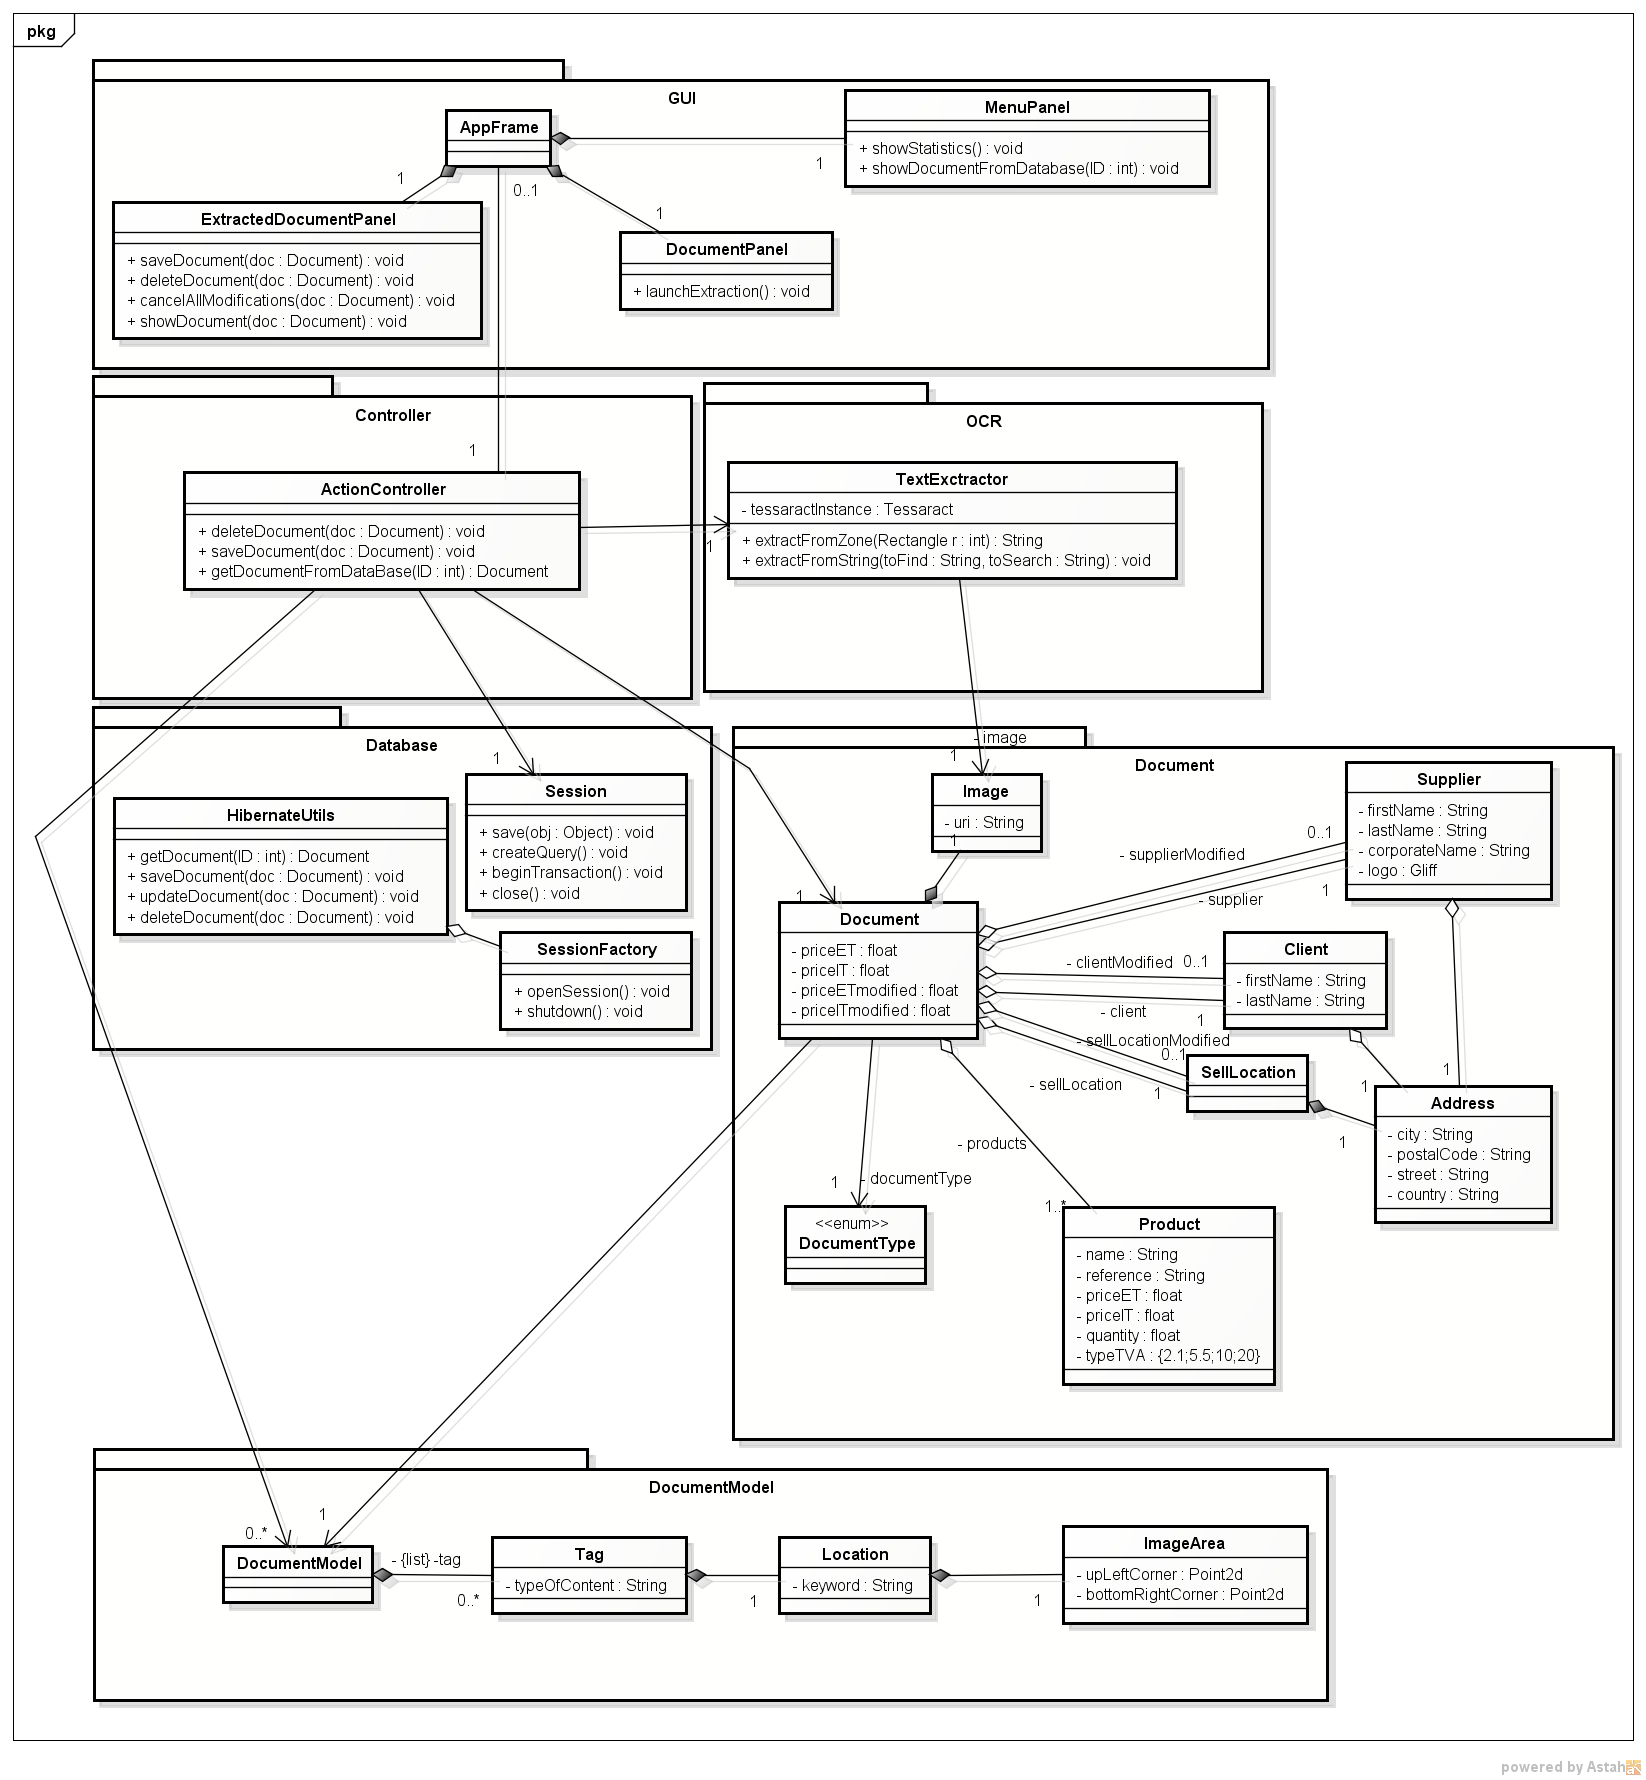
\includegraphics[scale = 0.3]{img/classDiag.png}
	\end{center}
	\caption{\it Diagramme de classe détaillé}
	\label{classDiagDetailled}
\end{figure}

\begin{itemize}
	\item[{\bf ActionController :}] L'entité ActionController a accès à tout. Elle utilise la classe TextExtractor situé dans le package OCR et une instance de DocumentModel situé dans le package DocumentModel afin d'extraire les données de l'image. Elle met à jour les valeurs du document courant et répond aux signaux envoyés par le GUI. Elle communique également avec la base de donnée du package Database pour le téléchargement et la sauvegarde d'informations.\\
	
	\item[{\bf TextExtractor :}] La classe TextExtractor va permettre tous les traitements à partir d'une image pour obtenir des String. Elle utilise une instance de Tesseract la librairie OCR et dispose de fonctions qui vont lui permettre de récupérer des données dans une zone de l'image, à partir d'un mot clé.\\
	
	\item[{\bf DocumentModel :}] La classe DocumentModel représente la manière dont on doit récupérer les données d'une image et leur attribuer un sens. Pour ce faire, il contient une liste de tags. Les tags vont correspondre à une location soit aussi une zone de l'image à traiter et un string correspondant à un mot-clé.\\
	
	\item[{\bf Document :}] C'est l'entité qui va permettre de regrouper tous les champs dont peut être composé une facture ou un ticket de caisse soit le DocumentType, le lieu de vente, le client, le fournisseur, les produits. Deux variables pour chacun de ces champs existeront dans le document, dans le but de stocker les données extraites mais également les données modifiées. Le document stockera aussi une image.
 \end{itemize}
 
 

\subsection{Diagramme de séquence détaillé}

\newpage

\begin{figure}[!h]
	\begin{center}
		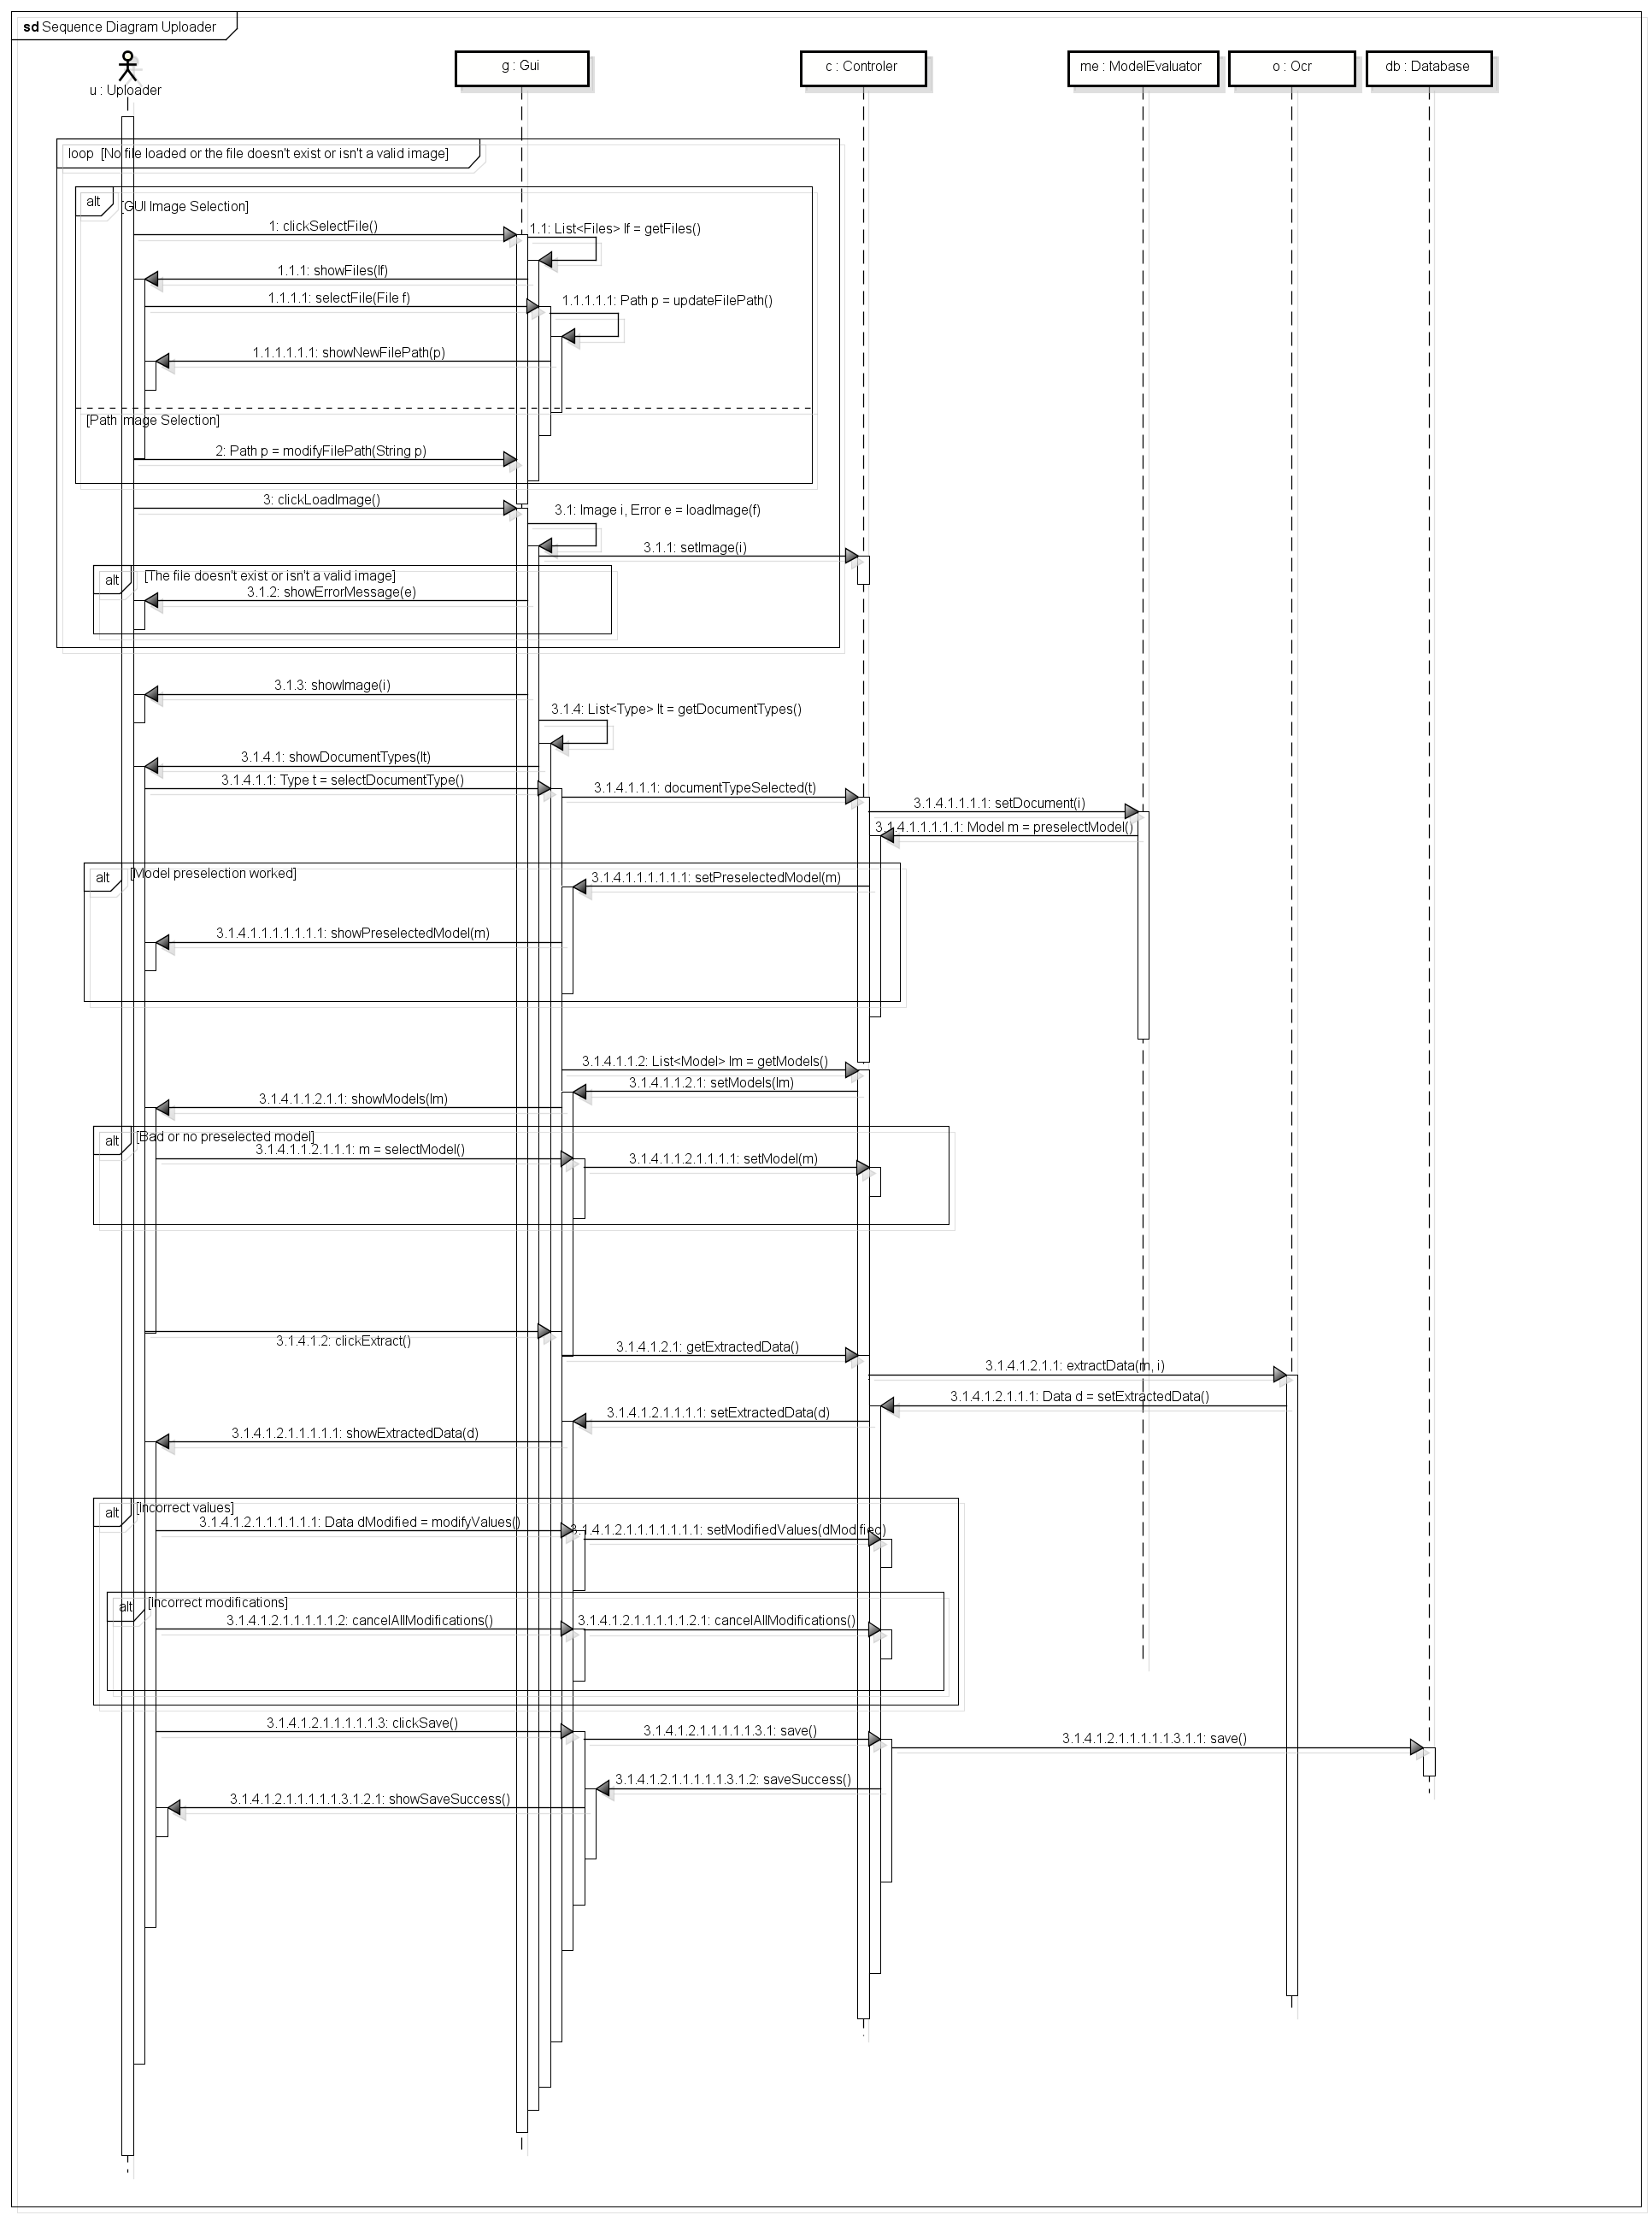
\includegraphics[scale = 0.3]{img/globalSeqDiagDetailled.png}
	\end{center}
	\caption{\it Diagramme de séquence détaillé - Uploader}
	\label{seqDiagGlobalDet}
\end{figure}

\newpage

\begin{itemize}
	\item[{\bf UID :}] sd3
	\item[{\bf Nom :}] Diagramme de séquence détaillé Chargeur
	\item[{\bf Resumé :}]  Charge une image et applique l'extracteur OCR pour remplir les champs appropriés. Les champs peuvent être modifiés et enregistrés dans la base de données.
	\item[{\bf Acteurs :}] Chargeur
	\item[{\bf Initiateur :}] Chargeur
	\item[{\bf Pré-conditions :}]  /
	\item[{\bf Post-conditions :}]  /
		\smallbreak
	\item[{\bf Description :}]
	Les fonctions propres au choix et vérifications du fichier getFiles(), showFiles() et selectFiles() sont prises en charges par l'interface elle-même. Elle est chargée d'afficher l'arborescence permettant la sélection du fichier à ouvrir. La fonction showNewFilePath() inscrit seulement le chemin du fichier sélectionné dans le champs correspondant. Le chemin peut également être entré manuellement.
	\medbreak
	Au chargement de l'image, une double vérification est effectuée : le fichier indiqué par le chemin existe-t-il , et le format de ce fichier est-il supporté par le programme. Si ces deux conditions sont vérifiées, l'image s'affiche; sinon, un message d'erreur informe l'utilisateur du problème rencontré.
	\medbreak
	Le système pré-sélectionne un modèle à travers le Controller via preselectModel() et la classe ModelEvaluator, et le présente à l'utilisateur grâce à la méthode showPreselectedModel() de l'interface.
	Celui confirme ou remplace le modèle puis clique ensuite sur le bouton "Extract". 
	\medbreak
	La fonction extractData() applique l'algorithme d'OCR grâce aux informations fournies par le modèle afin de remplir un maximum de champs. Les valeurs des champs sont affichées et peuvent potentiellement être modifiées par l'utilisateur puis enregistrées. Une modification va mettre à jour les données du document correspondant contenu dans la base de données. L'utilisateur peut également enregistrer simplement le document, ou supprimer un document existant. Le package Controller envoie systématiquement les informations à enregistrer au DataBase package. Un message confirme à l'utilisateur que l'action qu'il vient d'effectuer s'est bien déroulée.
\end{itemize}


\begin{figure}[!h]
	\begin{center}
		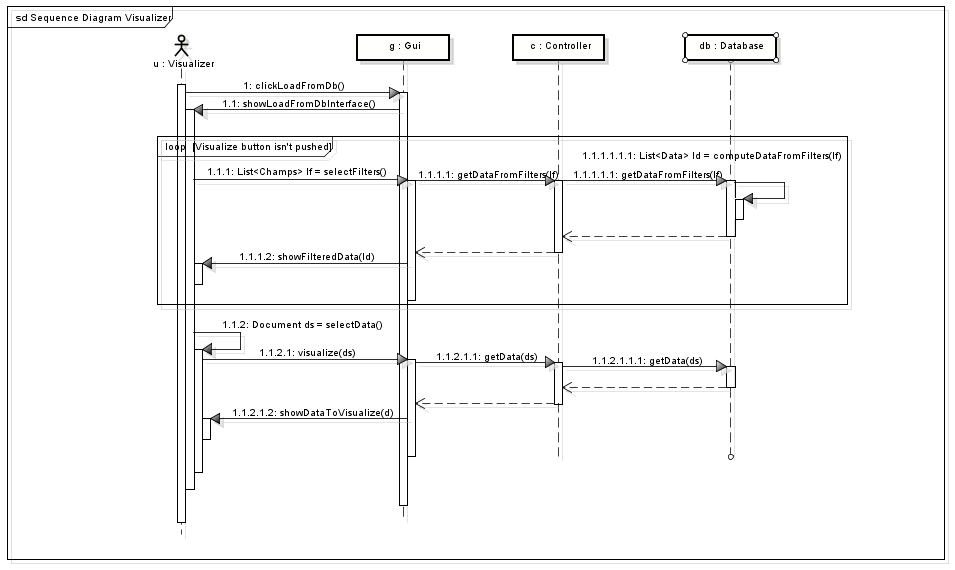
\includegraphics[scale = 0.6]{img/SeqDiagVisualizerDetailled.png}
	\end{center}
	\caption{\it Diagramme de séquence détaillé - Visualiseur}
	\label{seqDiagVisuDet}
\end{figure}

\newpage
\bigbreak

\begin{itemize}
	\item[{\bf UID :}] sd4
	\item[{\bf Nom :}] Diagramme de séquence détaillé Visualiseur
	\item[{\bf Résumé :}] Affiche un document provenant de la base de données.
	\item[{\bf Acteurs :}] Visualiseur
	\item[{\bf Initiateur :}] Visualiseur
	\item[{\bf Pré-conditions :}]  /
	\item[{\bf Post-conditions :}]  /
		\smallbreak
	\item[{\bf Description :}]
	Lors du clic sur le bouton "Load From DB", la fonction showLoadFormFbInterface() permet à l'utilisateur de filtrer les données de la base de données afin de sélectionner un fichier spécifique à visualiser. L'accès à la base de donnée est réalisé à travers les packages GUI, Controller et Database dans un sens et dans l'autre.
\end{itemize}

\bigbreak

\begin{figure}[!h]
	\begin{center}
		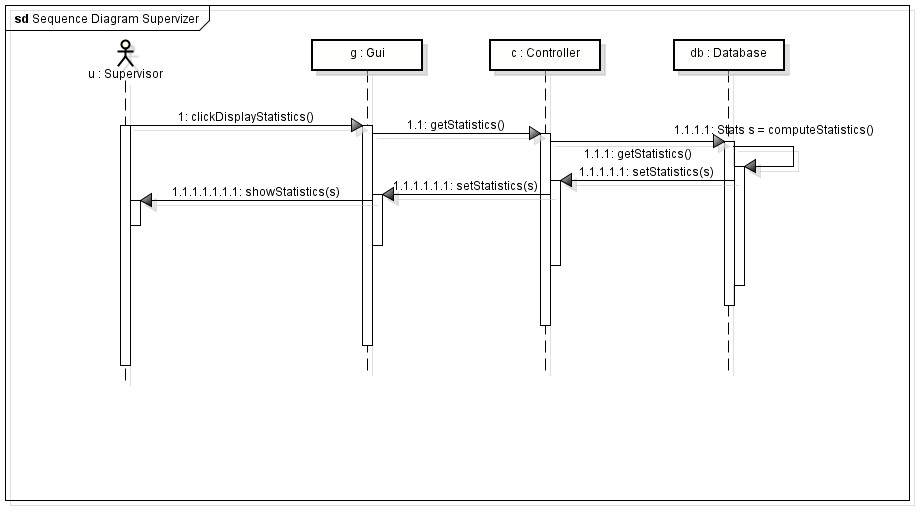
\includegraphics[scale = 0.6]{img/seqDiagSupervizerDetailled.png}
	\end{center}
	\caption{\it Diagramme de séquence détaillé - Superviseur}
	\label{seqDiagSuperDet}
\end{figure}

\newpage
\begin{itemize}
	\item[{\bf UID :}] sd5
	\item[{\bf Nom :}] Diagramme de séquence détaillé Superviseur
	\item[{\bf Résumé :}]  Charge une image et applique l'extracteur OCR pour remplir les champs appropriés. Les champs peuvent être modifiés et enregistrés dans la base de données.
	\item[{\bf Acteurs :}] Chargeur
	\item[{\bf Initiateur :}] Chargeur
	\item[{\bf Pré-conditions :}]  /
	\item[{\bf Post-conditions :}]  /
	\smallbreak
	\item[{\bf Description :}]
	La fonction clickDisplayStatistics() répond au clic de l'utilisateur cherchant à obtenir des informations sur les données stockées. La commande est transmises par le GUI package, puis le Controller package pour enfin arriver au DataBase package, après quoi le résultat parcours le chemin inverse pour permettre l'ouverture d'une fenêtre présentant les données statistiques à l'utilisateur.
\end{itemize}

